%%%%%%%%%%%%%%%%%%%%%%%%%%%%%%%%%
% 2022-01-22 ah - last revision 2022-05-29 15:15 CET ah
\documentclass[twoside,11pt]{article}
% Any additional packages needed should be included after jmlr2e.
% Note that jmlr2e.sty includes epsfig, amssymb, natbib and graphicx,
% and defines many common macros, such as 'proof' and 'example'.
%
% It also sets the bibliographystyle to plainnat; for more information on
% natbib citation styles, see the natbib documentation, a copy of which
% is archived at http://www.jmlr.org/format/natbib.pdf

% Available options for package jmlr2e are:
%
%   - abbrvbib : use abbrvnat for the bibliography style
%   - nohyperref : do not load the hyperref package
%   - preprint : remove JMLR specific information from the template,
%         useful for example for posting to preprint servers.
%
% Example of using the package with custom options:
%
% \usepackage[abbrvbib, preprint]{jmlr2e}

\usepackage{jmlr2e}
\usepackage{bm}
\usepackage{verbatim}
\usepackage{amsmath}
\usepackage{array, multirow}
\usepackage{graphicx}
\usepackage[colorinlistoftodos]{todonotes}
\usepackage{booktabs}

\usepackage{makecell}%To keep spacing of text in tables
\setcellgapes{4pt}%parameter for the spacing

% Definitions of handy macros can go here

\newcommand{\dataset}{{\cal D}}
\newcommand{\fracpartial}[2]{\frac{\partial #1}{\partial  #2}}
\DeclareUnicodeCharacter{2212}{−}


\usepackage{xcolor}
\usepackage[normalem]{ulem}
\newcommand{\addtxt}[1]{{\textcolor[rgb]{0.0,0.5,0.25}{{ #1}}}}
\newcommand{\sd}[1]{\textcolor{red}{[#1 \textsc{--Srijita}]}}
\newcommand{\MET}[1]{\textcolor{blue}{MET: #1}}
\newcommand{\AH}[1]{\textcolor{green}{AH: #1}}
\newcommand{\ytp}[1]{\textcolor{orange}{Tianpei: #1}}
\newcommand{\MO}[1]{\textcolor{red}{Mohammad: #1}}


% Heading arguments are {volume}{year}{pages}{submitted}{published}{author-full-names}

\usepackage{lastpage}
\jmlrheading{21}{2022}{1-\pageref{LastPage}}{3/22; Revised
x/22}{X/22}{20-212}{Retzlaff, Saranti, Angerschmid, Mousavi, Das, Wayllace, Afshari, Taylor, Holzinger}

% Short headings should be running head and authors last names

\ShortHeadings{Human-in-the-loop Reinforcement Learning}{Retzlaff, Saranti, Angerschmid, Mousavi, Das, Wayllace, Afshari, Yang, Taylor, Holzinger}
\firstpageno{1}

% added to fix Todolist error 
\setlength {\marginparwidth }{2cm}

\begin{document}

\title{Human-in-the-loop Reinforcement Learning: A Survey of Requirements, Challenges and Opportunities}

\author{\name Carl Orge Retzlaff \email carl.retzlaff@human-centered.ai\\ 
\addr Human-Centered AI Lab, University of Natural Resources and Life Sciences Vienna, Austria\\
and DAI Lab, TU Berlin, Germany\\
\AND
\name Srijita Das\email srijita1@ualberta.ca \\
\addr Department of Computing Science \\ 
University of Alberta, Canada
\AND
\name Christabel Wayllace\email wayllace@ualberta.ca \\
\addr Department of Computing Science \\ University of Alberta, Canada\\
\AND
\name Payam Mousavi \email payam.mousavi@amii.ca \\
\addr Alberta Machine Intelligence Institute\\
\AND
\name Anna Saranti \email anna.saranti@human-centered.ai \\
\addr Human-Centered AI Lab, University of Natural Resources and Life Sciences Vienna, Austria\\
\AND
\name Alessa Angerschmid \email alessa.angerschmid@human-centered.ai \\
\addr Human-Centered AI Lab, University of Natural Resources and Life Sciences Vienna, Austria\\
\AND
\name Mohammad Afshari\email mafshari@ualberta.ca \\
\addr Department of Computing Science \\ University of Alberta, Canada\\
\AND
\name Tianpei Yang\email tianpei.yang@ualberta.ca \\
\addr Department of Computing Science \\ University of Alberta, Canada\\
\AND
\name Matthew E.~Taylor \email matthew.e.taylor@ualberta.ca \\
\addr Department of Computing Science\\
Alberta Machine Intelligence Institute\\
University of Alberta, Canada
\AND
\name Andreas Holzinger \email andreas.holzinger@human-centered.ai \\
\addr Human-Centered AI Lab, University of Natural Resources and Life Sciences Vienna, Austria \\
and xAI Lab, Alberta Machine Intelligence Institute\\
University of Alberta, Canada
}


\editor{N.N.}

\maketitle

\newpage

\begin{abstract}%
Artificial intelligence (AI) in general, and reinforcement learning (RL) in particular, holds the promise of agents learning autonomously to accomplish difficult task with superhuman performance. However, even when an agent is going to eventually perform its task autonomously, we argue that RL is fundamentally a human-in-the-loop paradigm. For instance, an RL agent learns to act in a Markov decision process (MDP), but it is a \emph{human} who both sets an agent to act in this setting and specifies the MDP. Without a human, the agent would have \textit{no concept} of what a reward is or how to define it.  

This article argues that existing work in the literature has not adequately acknowledged this human-centrality as a key component to successful RL. Moreover, we show how significant improvements to existing explainability techniques are required to fully invest humans, whether lay people, subject matter experts, or machine learning experts, with the ability required to drive this human-agent interaction for Human-In-The-Loop (HITL) RL.

To subsume the central insights from this article, Table \ref{table:Explanations_table} gives an overview of the different phases for the agent deployment, with their respective requirements, aspects of human involvement, explanation types and new challenges. 

Our expectation is that readers of this article will understand (and ideally agree with) our argument that RL is fundamentally a human-agent interactive process. Furthermore, they will quickly understand what current state-of-the-art explainability methods can be used in HITL RL, be able to identify low hanging fruit on explainability research in RL, and appreciate longer-term research goals required to bring this field to fruition. We propose the vision of a human-robot teamup that allows both humans and robots to realize their full potential and play to their respective strengths.


\end{abstract}


\begin{keywords}
Reinforcement Learning, Human-in-the-loop, Explainable AI, Embodied Intelligence, Explainability
\end{keywords}


\section{Introduction}
\label{sec:introduction}

%RL = autonomous learning
%But, really humans involved throughout
%1) where humans interface with RL and 2) why explainability is critical
%Selecting algorithm, parameters, designing MDP, etc.
%Pretraining/incorporating knowledge in features, etc.
%Interactive teaching (curriculum learning), designing when to change MDP/agent (return to previous step)
%Decision to deploy: trust, safety
%During deployment: re-training, stopping, returning to drawing board
%
%Point of this article
%1) RL is human-in-the-loop
%2) Explainability is critical
%3) What we can do, what should do next (low hanging fruit), what's a long way off still


Reinforcement learning~\citep{SuttonBarto:2018:RLIntroduction} (RL) is a very general framework where an agent can autonomously learn how to take actions in order to best maximize the discounted long term sum of rewards. RL agents have had many impressive successes, such as in board games, video games, robotics and natural language processing \citep{Li:2017:DRLSurvey}. One of the benefits of RL is that agents can learn to outperform humans, sometimes coming up with completely novel (and unanticipated) strategies.

The RL paradigm seems to fit well with the long-standing goals of artificial intelligence, in that agents can go into an environment and autonomously learn how to solve difficult problems. However, we argue that this framing is naive, overlooking the significant human input and biases that are encoded into every RL problem. This article argues that: 
\begin{center}
\fbox{
    \parbox{0.95\textwidth}{
         \begin{enumerate}
            \item Reinforcement learning is fundamentally a human-in-the-loop paradigm and 
            \item Explainability is critical for the success of real-world \\reinforcement learning systems.
        \end{enumerate}
     }%
}
\end{center}

First, we argue that RL is a human-in-the-loop (HITL) paradigm, and identify four stages where human involvement is critical towards the goal of deploying and using RL agents. We emphasize that those stages are of cyclic nature and only loosely ordered in the presented sequence, meaning that the individual phases can be repeated and reiterated during the entire process of deployment.

% The development phase is characterized by the software and systems experts laying the technical groundwork. Here, the focus lays on the RL model itself.
% Then, the model is trained in an interactive fashion with an end user, under close supervision of the developers. This phase focuses on understanding the model perceptions and fundamentals, and evaluate the interaction with the end user.
% The third phase is characterized by testing the behavior of the trained model, which requires tools that allow to thoroughly evaluate a large-scale model. We will later talk about this fundamental challenge of finding explainable AI methods that scale well enough to support this phase.
% Finally, the model is deployed in the real world and interacts with the end user. The model now has to build trust with the end user by providing explanations for its behavior and still accommodate the efficient interaction expected for expert-level users. 

\vspace{2mm}
\emph{1: Initial Agent Development}

The agent's environment is first selected by a human based on where they think an RL agent might be useful, defining the problem to be solved. For that, human machine learning and/or subject matter specialists construct a Markov decision process (MDP), defining the state space, action space, and reward function --- all three have a critical impact on the speed of learning, the agent's final performance, and what policy is learned. They furthermore set the agent's algorithm and hyperparameters, and decide whether to incorporate prior knowledge, such as by adding detailed features or transferring knowledge from an existing agent. It must also be decided whether the agent should pre-train on existing data (e.g., using offline RL).
\vspace{2mm}

\emph{2: During Agent Learning}

Humans can decide to disallow the agent from selecting invalid actions or actions that are known to always be suboptimal. The agent's action selection can also be expanded with a bias by an expert to  enable faster learning rates. Furthermore, the developers can decide to include interactive paradigm with human demonstration, feedback, advice or other assistance.
Eventually, the subject matter expert should decide if the learning process is ``working well,'' or if the MDP should be revised, either because the agent is learning too slowly, or because the policy being learned is not what was anticipated for the problem.
\vspace{2mm}

\emph{3: Agent Evaluation}

The trained agent is tested by developers and subject matter experts.
The developers need to ensure that no erroneous behavior or glitches have emerged during training, operating mostly on a syntactical level. The subject matter expert will need to understand and evaluate the learned policies for sensible micro- and macro-behavior, constituting an evaluation of the semantic behavior. The decision for moving forward with the deployment to market or engaging in another development-learning-evaluation cycle lies in the evaluation phase and is made by the developers and project owners. The subject matter expert must decide if the learned policy is ``good enough'' to deploy, if more training is needed, or if the problem definition needs to be changed. 
\vspace{2mm}

\emph{4: Deployment of Learned Agent}

A human will typically need to argue why the agent is safe enough, or should be trusted enough, to be deployed in the real world. The deployment decision needs to be taken again by the end user, who determines the usage context and specific application of the agent in the field. Furthermore, the development team will need to determine if the agent should continually learn, if its policy should be frozen, or if it should retrain if the environment has changed ``enough.'' 
\vspace{2mm}

\begin{figure}[h]
    \centering
    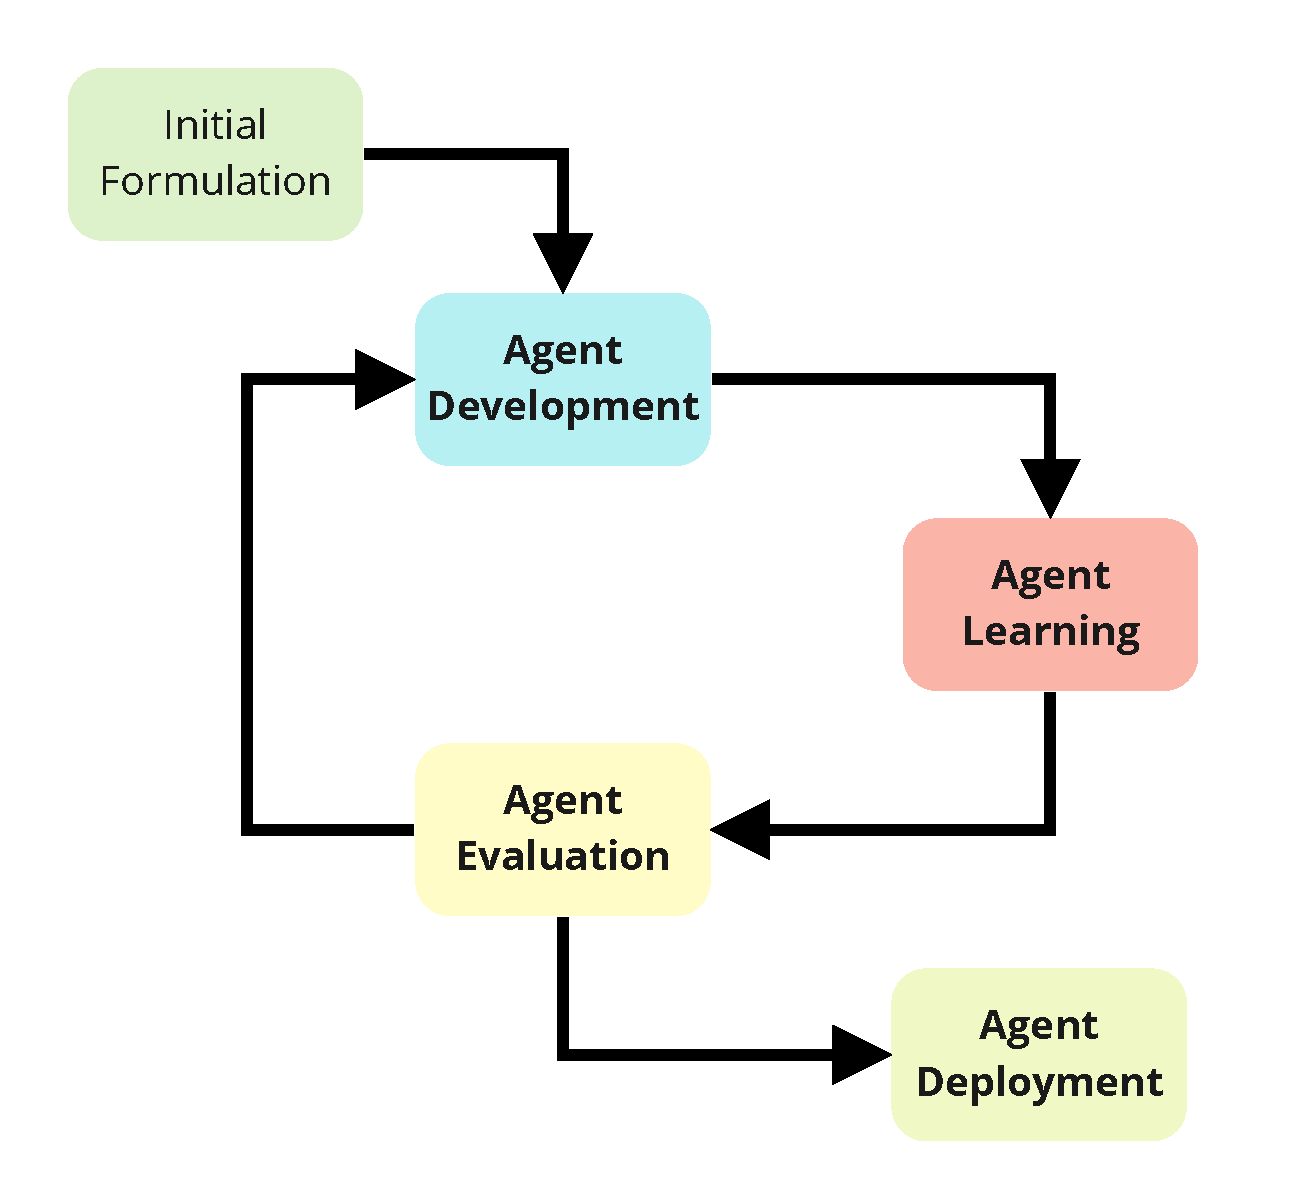
\includegraphics[width=0.6\textwidth]{img/HITL_Deployment_Workflow.pdf}
    \caption{Overview of the four steps to deployment and their sequence.}
    \label{fig:Deployment_Workflow}
\end{figure}

Figure \ref{fig:Deployment_Workflow} gives an overview of the different steps for the agent deployment and their sequence.

Second, in each of these four stages, we argue that explainability is a critical and underdeveloped technology. Before training, explainability can help show the impact of algorithm or hyperparameter selection, how prior knowledge biases the agent, and how pre-training changes the agent's learning process. During training and testing, explainability can show the impact biasing via an existing controller or human advice, how learning is progressing, or how the current policy functions. In the deployment phase after training, explainability can help explain the final policy, improve trust, help the person evaluate safety, and understand the policy's stability.

Part of this article can be considered as a position paper. We want to convince the reader that ignoring humans and treating RL as a fundamentally autonomous learning paradigm is shortsighted --- we will highlight where and how explainability can play a critical role is this human-agent collaboration. 

But this article can also be considered a survey. While discussing existing literature on explainability in RL, we will call out three types of challenges, and frame them as generations of technologies to emphasize future developments and the steps needed to take to achieve the larger goal of human-in-the-loop RL. Solved challenges are those where current explainability techniques can be used to help humans interact with learning agent, which reflect the current generation of technology. Short-term challenges are where we could easily adapt or extend existing explainability work to assist humans and belong to the second generation. Long-term challenges are those where significant research is required before a breakthrough can be achieved. This third generation of long-term challenges challenges are discussed extensively in Subsection \ref{sec:ThirdGeneration}.

The goal in this article is therefore both to try to shift the discussion about RL in general with respect to human subject experts, machine learning experts, or lay people, and also to provide an entry point into this exciting area of contemporary research at the intersection of explainability on RL, with the goal of getting non-experts quickly up to speed on exciting research directions. Throughout, we focus on human-robot interaction and therefore touch strongly on topics concerning embodied intelligence. But where appropriate, we will also refer to and discuss topics with regard to the respective superset of human-agent interaction. We furthermore differentiate between domain experts and end-users. We consider a person domain expert which is experienced in their respective field and has sufficient authority to be integrated as professional in the development cycle of a domain-specific product. End-users on the other hand are the customers which buy and use a final product. While they have a background in the respective field and are motivated to learn about the product, they could not provide guidance on designing such a tool.

The paper is structured as follows: After the introduction and motivation, we provide in Section \ref{sec:background} a thorough overview of background work for explainability and interactive learning and review fundamental and current challenges for embodied intelligence. Then, we explore the four stages for the deployment of HITL RL systems and analyze where to apply xAI in HITL RL Development (Section~\ref{sec:Developing}), Agent Learning (Section~\ref{sec:AgentLearning}), Evaluation (Section~\ref{sec:Evaluation}), and Deployment (Section~\ref{sec:Deployment}), each with specific requirements for the success of human involvement. Section~\ref{sec:discussion} discusses the general challenges observed and how future solutions can be shaped to overcome them. Finally, Section~\ref{sec:conclusion} outlines current problems and goals in the field and proposes further future work.

	\begin{table*}[!htbp]
	\tiny
	\resizebox{1\linewidth}{!}{
		\begin{tabular}{|c||l|l|l|l|}
			\cline{1-5}
			\multicolumn{1}{|c||}{ }  & \multicolumn{1}{c|}{ } & \multicolumn{1}{c|}{} & \multicolumn{1}{c|}{ } & \multicolumn{1}{c|}{ }\\
			\multicolumn{1}{|c||}{\textsc{Phase}}  & \multicolumn{1}{c|}{\textsc{Explanation Requirements}} & \multicolumn{1}{c|}{\textsc{Human Involvement }} & \multicolumn{1}{c|}{\textsc{Explainability} } & \multicolumn{1}{c|}{\textsc{Challenges}}\\
			\multicolumn{1}{|c||}{ }  & \multicolumn{1}{c|}{ } & \multicolumn{1}{c|}{} & \multicolumn{1}{c|}{ } & \multicolumn{1}{c|}{ }\\
			\cline{1-5}
			\multirow{11}{*}{\rotatebox{90}{\hspace{0em}\textsc{Development}}} 
			&  &  & & \\
			& $\cdot$Comparable between different model versions &$\cdot$Define Problem &\textbf{Techniques:} &	$\cdot$Creating Interactive, Thorough,\\
			& $\cdot$Rapidly Computable and&$\cdot$Construct State Space, &$\cdot$Pre-Training&$ $ and Comparable Model\\
			& $ $ Shallow OR &	$ $ Action Space,  	&	 $\cdot$Human-Readable Model 	&	$ $ Summaries	\\
			& $\cdot$Exhaustive but Slower &	 $ $ Reward Function 	&	 $\cdot$Policies 	&	$\cdot$Use Compositional and	\\
			&&	 $\cdot$Model Design 	&	 $\cdot$Causal Models	&$ $ Representational Language	\\
			&&	 	&	 \textbf{Directionality:}	&$\cdot$Integrate Causal Learning	\\
			&&	 	&	 $\cdot$Unidirectional (model to user)	& $\cdot$Use Policy Querying	\\
			&&	 	&	 \textbf{Users:}	&	\\
			&&	 	&	 $\cdot$RL Experts	&	\\
			&  &  & & \\
			\cline{1-5}
			\multirow{10}{*}{\rotatebox{90}{\hspace{0em}\textsc{Agent}} \rotatebox{90}{\textsc{Learning}}} 
			&  &  & & \\
			& $\cdot$Interpretable Inputs &	 $\cdot$Evaluative Feedback 	&	 \textbf{Techniques:} 	&	$\cdot$Start with Imitation Learning and	\\
			& $\cdot$Interactive&	$\cdot$Action-Advice 	&	 $\cdot$Perception Explanation 	&	$ $ Fine-Tune with Preference-Based 	\\
			& $\cdot$Support Human as Teacher &	 $\cdot$Human Preference 	&	 $\cdot$Behavior Evaluation 	&	$ $ Learning	\\
			& $\cdot$Understandable by&	 $\cdot$Demonstrations 	&	\textbf{Directionality:}   	&	$\cdot$Adapt xAI Approaches to HITL\\
			& $ $ Domain Expert & 	&	 $\cdot$Bidirectional 	&$ $ Context	\\
			&   & 	&	 \textbf{Users:}	&	$\cdot$Supporting Human as Teacher 	\\
			&   & 	&	 $\cdot$Domain Experts	&	$ $ with Replanning and Corrections	\\
			&   & 	&	 $\cdot$RL Experts	&	\\
			&  &  & & \\
			\cline{1-5}
			\multirow{10}{*}{\rotatebox{90}{\hspace{0em}\textsc{Evaluation}}}
			&  &  & & \\
			& $\cdot$Explanations of  & $\cdot$Understand and Evaluate	&	 \textbf{Techniques:}	& $\cdot$Ensure Understandability for	\\
			&  $ $ Learned Behavior & $ $ Learned Policies on Micro	&	 $\cdot$Policy Summarization	&$ $ Subject Expert	\\
			& $\cdot$Scale to Large Models  & $ $ and Macro-Level	&	 $\cdot$Graph-Based Explanations	&	$\cdot$Thorough and Comparable \\
			& $\cdot$Comparable to  & 	&	 \textbf{Directionality:}	& $ $ Explanations that Scale with	\\
			& $ $ Untrained Model  & 	&	 $\cdot$Bidirectional	& $ $ Model Size and Complexity	\\
			& $\cdot$Understandable by  & 	&	 \textbf{Users:}	& $\cdot$Dashboard for Inspection from 	\\
			&  $ $  Domain Expert& 	&	 $\cdot$Domain Experts	&$ $ Different Viewpoints/Aspects	\\
			&  $ $   & 	&	 $\cdot$RL Experts	& 	\\
			&  &  & & \\
			\cline{1-5}
			\multirow{10}{*}{\rotatebox{90}{\hspace{0em}\textsc{Deployment}}}
			&  &  & & \\
			&  $\cdot$Rapid Computation and& $\cdot$Deployment and	&\textbf{Techniques:}	&	$\cdot$New Approaches Beyond Image\\
			&  $ $  Low Cognitive Load& $ $ Usage Decision	&	 $\cdot$Combined Explainability	&$ $ and Driving-Based Explanations	\\
			&  $\cdot$Understandable by End-User& $\cdot$Interaction with End-User	&	 $ $ Dashboard	&	$\cdot$Simple and Fast Explanations\\
			&  & 	&	 $\cdot$Intent Communication	& $\cdot$Error and Uncertainty Handling	\\
			&  & 	&	 $\cdot$Error Handling	& $\cdot$Communication of Agent Intent \\
			&  & 	&	\textbf{Directionality:}	&$ $ Via Different Modalities	\\
			&   & 	&	 $\cdot$Bidirectional	&	\\
			&   & 	&\textbf{Users:}	&	\\
			&   & 	&	 $\cdot$End-Users	&	\\
			&  &  & & \\
			\cline{1-5}
		\end{tabular}
	}
	\caption{Overview of the different explanations contexts in the four different phases. \emph{Explanation Requirements} enumerates desirable properties of explanations at this stage, and \emph{Human Involvement} describes how the human is involved in it. The \emph{Explainability} column lists (1) example techniques currently used, (2) directionality of explanations, i.e., agent to human, human to agent, or both, and (3) the types of users interacting with the agent at this stage. The \emph{Third Generation Challenges} describes blue-sky propositions we envision for a comprehensive HITL RL experience.}
	\label{table:Explanations_table}
\end{table*}

We created  table \ref{table:Explanations_table} with the intention to give the reader a comprehensive overview of the main insights of our paper. It gives a synopsis of the central aspects of this paper, and subsumes the requirements, challenges and human context for the four phases we discuss extensively in the following pages. 

We want to show that RL greatly benefits from being thought of as human-centered process, and that explainability is required to enable this HITL RL approach. We aim to highlight how current xAI methods can be used to facilitate such HITL approaches, and identify low hanging fruits for further explainability research, ultimately enabling a more productive interaction of humans and RL agents.

% ==================
\section{Background}
\label{sec:background}

In the background section, we want to establish the technical backdrop for our discussion of the four phases of the deployment of HITL RL agents. We therefore detail the concept of explainability and essential approaches for facilitating insights into the workings of ML models. We then refer to interactive learning as  approach for integrating human-in-the-loop into RL by guiding the RL agent to leverage domain knowledge and rich human experience. Finally, we summarize current challenges for reinforcement learning in general and more specific to the HITL context.

\subsection{Explainability}

Explainable artificial intelligence (xAI) is a framework for helping human users understand the process and outputs of machine learning models. As ML models are deployed in a growing number of applications that affect human life (e.g., agriculture, forestry, health,etc.), the need for such xAI frameworks is ever more apparent. The xAI approaches are essential for many human-AI collaboration scenarios, where understanding and trusting the outputs of the model is a prerequisite for their use.  

Explainability has grown from the 1990's with researchers aiming to extract rules from neural networks \citep{TickleEtAl:1998:HistoryNN}, towards an progressively expanding, dedicated research community, as seen at the example of the DARPA initiative \citep{GunningAha:2019:DARPA}. The xAI efforts have since led to a number of very successful xAI methods \citep{HolzWoj:2022:XAIOverview, ZhouEtAl:2021:QualitySurvey}. Explainability in this context is a technical term used to refer to the collection of methods that aim to highlight decision-relevant parts of machine representations and machine models.

The following examples show how xAI frameworks and human users can interact:
\begin{enumerate}
\item Explaining the role of data source in the final decision. Specifically, to identify which data samples were used for a specific action or decision. This is also important for assigning credit to (and potentially compensating) the individuals who produced the data~\citep{zanzotto2019human}. 
\item Identifying and visualizing components of the model that contributed to its accuracy or to a particular prediction during training via a heatmap \citep{SturmEtAl:2015:InteractiveHeatmap}.
\item Building trust in the human users specifically when safety is a major issue. For example, in AI applications in medicine, the human user cannot blindly trust the decision made by the AI agent without a reliable explanation. Transparency and accountability are essential ~\citep{Schneeberger:2020:legalAI, Stoeger:2021:MedicalAI}. Hence, xAI strives for high-level of model correctness, helps with generalization and attempts to minimize confident decisions made based on faulty/inappropriate data. Other applications such as autonomous vehicles or robotics are additional examples of cases where the decisions have a significant impact on safety and therefore trust and accountability are pertinent~\citep{araiza2019safe, WellsBednarz:2021:xAIRLSurvey}.
\item Enabling humans to provide richer feedback through additional, optional counterfactual examples. The feedback, in the form of explanations provided by humans is used by the AI agents towards ultimately a two-way cooperation leading to ever more accurate, robust, and transparent models ~\citep{Karalus:2021:HITL-counterfactuals,PuiuttaVeith:2020:xAIRLSurvey}.   
\end{enumerate}

These examples show the diverse applications for xAI frameworks. However, objectively assessing the quality of xAI solutions is a key element for their successful deployment. \cite{milani2022survey} name four key metrics for evaluating xAI solutions: \emph{Fidelity}, the truthfulness of the explanation with regard to the model itself. \emph{Performance}, the default metric used to evaluate the success of the AI solution to be explained. \emph{Relevancy}, the relevance of the provided explanations to the task at hand, and \emph{Cognitive load}, the mental effort required to understand the provided explanations. \\

% Moved the section on interpretability here so we could use the same categorization for explainability as well (Payam) - Are we OK with this?

%I feel there is no flow between the previous and this paragraph - Chris

Interpretability can be considered a subset of explainability, and is defined as the methods which passively make the model understandable, whereas explainability actively generates explanations for a model. We refer to \cite{GlanoisEtAl:2021:SurveyInterpretableRL} for a comprehensive survey of interpretable RL, but extend their categorization of interpretability approaches to include explainability models as well. The three major categories are: 1) interpretable/explainable inputs of RL models, 2) interpretable/explainable transition and reward models for RL, and 3) interpretable/explainable decision-making processes of RL. 

The first category focuses on the inputs to the RL model used to make decisions. It not only includes the agent's state, but also other structural information, such as the problem descriptions from human experts \citep{hasanbeig2021deepsynth}, and the relational \citep{battaglia2018relational,martinez2017relational} or hierarchical structure \citep{andreas2017modular,lyu2019sdrl} of the problem. Such information helps humans better understand the decisions made by RL models. 
%Visualization
A prominent approach and important building block for explaining complicated inputs is to visualize them as the model perceives them. This is often combined with showing relevance and importance for model decisions, which can help to evaluate whether the model is looking at the right input aspects, but also has its own caveat of possibly misleading the user. See \citet{EvansEtAl:2021:ExplainabilityParadox} for further discussion.
In the broad approach of saliency maps, important image regions are highlighted. \citet{LiuEtAl:2018:LinearModelUTrees} show an example where continuous ``super-pixels'' with large feature influence are highlighted. \citet{Bach:2015:LayerWiseRelevancePropagation} develop the technique of ``Layer-Wise Relevance Propagation'', that iteratively changes the model inputs to find the relevance of individual (image) parts or features. \\

The second category exploits an interpretable/explainable model of the task or environment, e.g., a transition model \citep{martinez2016learning,zhu2020object} or a preference model \citep{icarte2018using,toro2019learning}. Such models help both the RL agent's reasoning about its decision-making and humans' understandings of the decision-making process. \\

The third category is the interpretable/explainable decision-making of RL agents, referring to cases where policies can be learned in a fully understandable manner. Some of the previous work directly learns such interpretable policies in the form of decision trees \citep{likmeta2020combining,silva2020optimization,topin2021iterative}, formulas \citep{hein2018interpretable,hein2019generating}, fuzzy rules \citep{akrour2019towards,hein2017particle,zhang2021kogun}, logic rules \citep{jiang2019neural}, programs \citep{sun2019program,verma2019imitation} and so on. Other researchers first learn a non-interpretable policy, then transform this policy to an interpretable one through imitation learning or transfer learning \citep{bastani2018verifiable,VermaEtAl:2018:ProgrammaticallyInterpretableRL}.

A subset of xAI methods go beyond explaining outputs of feed-forward models assuming \emph{independent and identically distributed} (i.i.d.), input data distributions to shed light on \emph{decisions} made by the models, often parameterized by and referred to as \emph{policies}. These models are therefore specific to RL. The following approaches are examples for xAI techniques specifically related to explaining policies (i.e., fit within the third category): 

%Policy Summarization
In policy summarization, the general aim is to make the underlying model and its policy tangible. This can be done via codifying its decision process as rules, as seen in the linear model u-trees by \citet{LiuEtAl:2018:LinearModelUTrees}. These networks aim to represent the Q-function and use it to make more transparent the feature influence and the rules learned by the network. 
Another approach is to represent the learned model with generated code blocks, as presented by \citet{VermaEtAl:2018:ProgrammaticallyInterpretableRL}. Their `Programmatically-Interpretable RL'' first learns a neural policy network and then searches a programmatic policy that adequately codifies this network. This approach incurs a performance degradation during training, but results in human-readable policies and improves generalization.
A third approach is to represent the network policies via natural language. \citet{AlonsoEtAl:2018:xAINLBeerClassifier} show an example of justifying classifications with a textual explanation of the choice made by a decision tree. 

The examples shown are sorted in descending order of complexity: the rule representation is the most technical, and code examples provide a middle ground between technical requirements and formal correctness. On the other hand, the representation with natural language is most intuitively understandable but also less exact.

%Policy Querying

In policy querying, the decision process leading to a given result is explained. This can be either general (``when do you do X'') or or specific to a given action/decision.
An example for a specific explanation is the natural language explanation for a classification as presented by \citet{AlonsoEtAl:2018:xAINLBeerClassifier}, when they provide a textual explanation along with additional details that show how individual factors where quantified and evaluated.
An example for general policy querying is presented by \citet{HayesShah:2017:AutonomousPolicyExplanation}, which generate a summary of a ``when do you do X?'' type question in natural language to explain the actions of an agent. \\


% Causal Learning subsection

A relatively new and fundamentally different approach to explainability is provided by causal models. Methods available within this framework, generally fall into the second and third categories as they aim to provide causal explanations for the task/environment or the policies respectively. Explainable AI methods that construct causal models, like probabilistic graphical models (PGM) \citep{Koller:2009:ProbabilisticGraphicalModelsBook, Saranti:2019:LearningCompetencePGMs} are slowly emerging in the international literature, 
partly due to the recognition that conventional machine learning models (including neural networks) base their decisions on correlations between input data and the desired action  \citep{Lapuschkin:2019:UnmaskingCleverHans}. 

% GNN
Another causal learning approach uses graph neural networks (GNN) \citep{Vu:2020:PGMExplainer}, to generate explanations for a prediction via a PGM that identifies crucial graph elements (e.g., nodes, edges) causally responsible for that prediction. Current work is also incorporating the human-in-the-loop strategy \citep{HolzingerEtAl:2016:iMLExperiment, Holzinger:2019:HumanLoopAPIN} where expert domain knowledge is used to select actions. 

% Use opportunity chains as modality for good explanations
\citet{MadumalEtAl:2020:CausalRLCFs} encode causal models using \emph{action influence graphs} to generate explanations using \emph{causal chains} resulting in better explanations as well as improved prediction performance. In their more recent work, \citet{Madumal:2020:DistalEF} propose that investigating interactions between RL agents and humans is the key to generating finer details in the explanations thus alleviating some of the shortcomings of the action influence models. An insight gained through their human studies was that to generate explanations, humans tend to refer to \emph{future} actions that were dependent on the current ones. This supports the idea that humans have a deep understanding of cause and effect chains of actions and events, often referred to as \emph{opportunity chains} in the cognitive psychology literature. Inspired by this, the authors create explanatory models that focus on these opportunity chains and the future actions, they call \emph{distal} action. 

% connection to HITL
\citet{LiangEtAl:2017:HITLReinforcementLearn} argue that the cognitive ability of the human operator paired with the computational power of a machine have the potential to handle complex tasks. Moreover, they state that it is essential for a productive interaction that the machine is able to react to the environment as well as the human operator. This was demonstrated by safety measurements showing that the machine needs to pay attention to the operator as well as the environment and possible bystanders. Furthermore, humans need to understand and interpret the actions of the machine correctly to improve the algorithm \citep{heuillet2021explainability}. Moreover, \citet{heuillet2021explainability} state that the underlying algorithm and its decisions need to be understandable for a multitude of different audiences with various goals.

% Counterfactuals

With the help of adequate personalized User Interfaces (UI) \citep{Sun:2021:TopologyPerturbationGNNs}, counterfactuals can also be created by following an action sequence driven by human expertise. This can also be injected in the form of the priors of the random variables and consists of a form of inductive bias.
Beyond counterfactuals, ``opportunity chains'' contain a sequence of events with causal dependency, and contain the concept of enabling events down this sequence \citep{Madumal:2020:DistalEF}.

% Not just use human explanations as prior, but use expertise to imitate
Observational data from expert actions go beyond injecting a prior to an explainable model \citep{Zhang:2020:CausalImitationLearning}. Causal imitation learning learns a structural causal model (SCM) \citep{Pearl:2000:ModelsReasoningInference} from policies performed by humans, even if the actual reward is not specified and the environment is not perceived the same to the learner and the human expert demonstrator. But this can also be beneficial since researchers have shown that incorporating that knowledge maximizes the aggregated reward, even if it sacrifices some autonomy. 

Dynamic SCMs are incorporated to formalize the partially-observable markov decision process (POMDPs) \citep{SuttonBarto:2018:RLIntroduction} as perceived by the agent, and take into account the human intervention and its implications. The so-called counterfactual agent does not blindly take the human's advice and execute it; it compares it with other possible actions and decides correspondingly. In cases where the reward and the transition functions are the same, the ``human-in-the-loop'' is beneficial, even if the human's instructions are far from perfect. The implications that this will have on the explainability of the learned models are a vital area of future research. Especially in the latter case, where the human needs to provide adequate instructions in selected states, the human understanding of the agent's current SCM, is vital.  

\subsection{Interactive Learning}
\label{sec:InteractiveLearning}
    
The most fundamental ways of learning in nature is parents teaching their off-springs in an interactive fashion. Similar learning dynamics exist between a teacher and a student, where the teacher tries to guide the student with their experience and knowledge. Following the same motivation, interactive learning~\citep{Arzate:2020:SurveyInteractiveRL} in RL aims to involve human-in-the-loop to guide the RL agent by leveraging domain knowledge and rich human experience. In recent times,  RL has been successfully applied to solve many real-world problems, ranging from drug discovery~\citep{popova2018deep}, navigating super pressure balloons in the stratosphere~\citep{bellemare2020autonomous} to robot manipulation tasks~\citep{nguyen2019review}. While this is an exciting direction for research, recent deep RL systems still face a lot of bottlenecks, including sample inefficiency, sim-to-real transfer issues, generalization, exploration, etc., to name a few~\citep{ibarz2021train}. Interactive RL aims to solve some of these challenges by involving a human prior to training~\citep{Guo:2022:RLSurveyHumanPriorKnowledge}, during training~\citep{Knox:2008:TAMER} or in the deployment phase of the RL system~\citep{guo2021edge}. Interactions could either be teacher-initiated~\citep{torrey2013teaching}, student-initiated~\citep{da2020uncertainty,MandelEtAl:2017ActionsInHITL} or jointly initiated~\citep{amir2016interactive} by both the parties.

In interactive learning, the human is characterized as a teacher and the teaching loop can contain different types of critique, advice modalities and guidance that can be fed back to the RL algorithm. There can be different modalities of human advice such as binary evaluative feedback [+1/-1] ~\citep{Knox:2008:TAMER}, action-advice~\citep{torrey2013teaching}, preference based feedback~\citep{Christiano:2017:DeepRLHumanPreferences,LeeSmithAbbeel:2021:FeedbackPreferenceHITLLearningPEBBLE}, and sub-goal specification~\citep{le2018hierarchical}. A comprehensive survey of various types of human guidance in Deep RL can be found in \citet{zhang2019leveraging}. \citet{Thomaz:2006:RLWithHumanTeachers} proposed one of the earliest work on Interactive RL which allowed human trainers to give binary feedback for the agent's behavior and specific objects associated with the task. \citet{Arzate:2020:SurveyInteractiveRL} showed that humans provided rewards for future actions rather than past actions executed by the agent  classify methods of interactive RL according to the way human feedback tailors an RL dimension. That method could modify the reward function, the agent's policy, the exploration process, or the value function.  

A common approach to modify the reward function is called reward shaping. In reward shaping, the teacher provides useful information to shape the reward function so that favourable parts of the state-space are encouraged and unfavourable parts are penalized \citep{ng:99}. This is useful in sparse reward environments and facilitates the reward specification in complex domains. A well-known reward shaping framework is TAMER~\citep{Knox:2008:TAMER, knox:13} where the human provides evaluative reinforcement (positive or negative feedback) by observing the agent in action. This signal is used to build a model of the human's reward function. 

Methods that consider modifying the agent's policy are called policy shaping \citep{cederborg2015policy,griffith2013policy,WuEtAl:2021:HITLDRLAutonomousDriving}. These methods augment an agent's policy directly using human knowledge. This technique does not require a well formulated reward function, but it assumes the trainer knows a near-optimal policy to guide the agent. \citet{macglashan2017interactive} proposed COACH framework and showed that human feedback is dependent on the agent’s current policy. 

Human advice can also be useful in guiding the agent in it’s exploration phase so that the high rewarding states or trajectories are identified by the agent in less number of environment interactions~\citep{amir2016interactive}. Action pruning is another way where human-in-the-loop RL can guide exploration and improve learning \citep{Abel:2017:AgentAgnosticHumanInTheLoopRL}.

Lastly, human-advice-based value functions can be combined with agent value functions~\citep{jiang:21,kartoun:10, taylor2011integrating, WuEtAl:2021:HITLDRLAutonomousDriving} to effectively guide the agent. Demonstrations \citep{hester2018deep,vecerik2017leveraging,nair2018overcoming} from humans can also augment the value function by biasing it according to the  actions taken by the expert. These approaches have been particularly successful in complex robotics tasks like pushing, sliding etc which can easily be demonstrated by humans.  Demonstrations, by default, may contain human biases which can, in turn, be removed by experts \citep{Wang:2022:SkillPreferences}.

The first indicator for the need for human intervention is model performance, since a bad model is more likely to produce bad policies. However, good models can also lead to bad policies as well at deployment scenarios because of the sim-to-real gap. In many cases, human intervention is simulated from pseudo-agents since both the potential benefits and the need to know where the imperfections of the model are can be detected before deployment. The designer of the interactive framework must also take into account that the human interventions might not always be perfect or beneficial; the user might need special training and an informative user interface to effectively improve the RL algorithm. 
%merged the UI paragraph from the Interactive learning section here

The type of UI, hardware-delivered or natural interaction,  determines the degree of expertise required and can affect the quality of the feedback \citep{lin:20}. Keyboard keys, mouse clicks with sliders, and game controllers are examples of UIs in hardware-delivered interactions, and experts or knowledgeable trainers generally use these UIs. On the other hand, sound interfaces that use the techniques of audification and sonification \citep{Hermann:2011:Sonification,kartoun:10, Saranti:2009,Scurto:2021:DesigningDeepRLHumanParameterExploration}, cameras to capture facial expressions \citep{arakawa:18}, etc. are examples of UIs for natural interaction that non-expert users prefer. 

\subsection{Challenges for Reinforcement Learning and HITL approaches} 
\label{sec:ChallengesRL}

To conclude the background section, we want to talk about underlying challenges for reinforcement learning in general and those more specific to HITL approaches in order to get a better understanding of fundamental and current challenges in the field.

%%%Exploration Exploitation Tradeoff
One fundamental challenge is the Exploitation Exploration trade-off. The trade-off is defined by the decision when to continue exploiting a current option, and when to explore further for new options. This challenge is most often illustrated at the example of the one-armed bandit. An agent is tasked with finding the best (ie. most rewarding) one-armed bandit slot machine in a casino, and has a limited amount of coins. When the agent is now sitting at machine A, how long does he take to evaluate whether this machine provides a higher payoff, and when does he cut his losses to move on to another automaton? A more in-depth description of this problem can be found in \citet{AudibertMunosSzepesv:2009:ExplorationExploitation}.

%%%Reality Gap
Another general challenge is the ``sim-to-real gap'', which describes the difficult task of translating the experience from a simulation to an applications reality \citep{ZagalJavierVallejos:2004:RealityGap}. It first implies that we are always under-modelling our system, which means that aspects of reality are missing which will present our agent with unforeseen challenges and sometime even prevents a policy learned in a simulation from being transferable to the real world. Secondly, real-world samples are very expensive (cost, complexity and time-wise), which makes modelling despite its challenges much more appealing  \citep{KoberBagnellPeters:2013:RLRoboticsSurvey}.

%%% Pixel based learning is hard and leads to brittle assumptions
With vision being a central modality for agents employed in the real world, learning from pixels is essential. This is however a very hard problem, which often relies on brittle assumptions and in consequence often does not generalize \citep{TomarEtAl:2021:LearnPixelControlRepresentations}.


More specific to reinforcement learning for embodied intelligence, \citet{RoyEtAl:2021:RLRoboticsChallenges} provide a comprehensive overview of different challenges. To highlight five constraints particular to it:
\begin{itemize}
    \item Interaction with real world entails safety risks for exploration and hard limits on resources like energy.
    \item Poor alignment of learned models and real world.
    \item Require stronger generalizations  and adaptation since specifications, goals and rewards might change.
    \item Observed data is plentiful but drawn from local distribution, requiring agent to learn a reasonable world model beyond  what is currently observed. 
    \item Agent morphology defines what can be learned from the environment and has to be considered when designing agents.
\end{itemize}

Partially overlapping with those constraints, \citet{ibarz2021train} conducted a survey of RL applications and some of the main challenges they identified were sample efficiency, sim-to-real-gap, exploration challenges, generalization challenges, goal and reward shaping and safety issues. Finally, there are challenges more specific for HITL approaches. 

%reward shaping is difficult
To be able to characterize, describe and compare reward shaping approaches, one needs some xAI methods to uncover the rules by which the neural network decides for an action. The designer or RL systems is there to provide the basic framework parameters - the most fundamental of those being the reward scheme - but a deeper interference can eventually destroy the potential of the agent being able to figure out effective strategies on its own. The challenge is that the cost/reward function design needs domain knowledge, but does the human always (at each possible state) know what is a profitable behaviour? The main idea is to not shape the reward too much or make it too complex --- but those two are highly subjective and need to be tested in practice. So, apart from the exploration-exploitation balance, there is also a trade-off between human intervention and the agent's ability of invention (intervention-invention). The main research question is to what extend should RL imitate a good human player or expert, and how can RL with the human-in-the-loop can discover new action sequences, not yet thought by humans and how xAI can help bridge this divide. \citet{LeeSmithAbbeel:2021:FeedbackPreferenceHITLLearningPEBBLE} discuss this challenge for reinforcement learning and propose a HITL approach to deal with this.

% when did training converge and when to include human
Deep RL agents, after training has reached a good performance, will generalize best for good players. However, we know that explanations are not reliable and do not make sense when the neural network does not have an overall good performance or generalization capability, even more for misclassified examples or other underlying errors. Therefore it is difficult to think in what way one can use those explanations during the training process or how one could automate the process of finding the right time point (epoch) to allow the human to do so. Newer methods for RL, like HindsightExperienceReplay (HER) \citep{Andrychowicz:2017:HERHindsightExperienceReplay}, even consider episodes where the goal state is not reached as such to use this additional information. This is more likely in a neural network that is not trained to the extent of having a good enough performance. In such a scenario, adequate xAI methods could shed light on agents that follow RL-policies with several goals. 

%limits of xAI?
One other aspect is that most of the current xAI methods invented for deep neural networks that also have a practical implementation are not created with RL principles in mind. They are typically created with the intent of uncovering a simpler, interpretable model or to pinpoint the important elements of a potential input, driven by the mathematical principles of neural networks. For example, in the groundbreaking example of the convolutional neural network (CNN) that was used to process the Atari images \citep{Mnih:2013:PlayingAtariDeepRL} a state-of-the-art xAI method, namely layer-wise relevance propagation (LRP) could be used \citep{Bach:2015:LayerWiseRelevancePropagation,Alber:2019:Innvestigate}. However, this would only provide to the user a heatmap about what is positive and what is negatively relevant for the prediction, meaning that it would only characterize (in RL terms) one input state. Those heatmaps are not juxtaposed or combined with the possible actions from that state, or their expected reward as a whole ---the human would not know why the RL algorithm decided for the selected next action. To reconstruct the complete strategy of a model, its rules and the underlying purposes of all (or at least the representative) state-action pairs out of those heatmaps, would be a very cumbersome task. 

We argue that the discussed challenges show that generalisable and performant RL is a fundamentally challenging problem, as exemplified by the different obstacles detailed in this Section. We claim that many of those challenges can be overcome with the application of HITL approaches. 
% Similarly, \citet{MatthewsonPilarski:2022:DesigningAndEvaluatingHCIML} argue that human-centered thinking for RL approaches is essential for designing and deployment of RL systems, enabled by human-centered approaches like reward shaping and better feedback between agent and human \citep{Li:2019:HumanCenteredRLSurvey}. While \citet{MatthewsonPilarski:2022:DesigningAndEvaluatingHCIML} take the bird-eye perspective on all machine learning as interactive machine learning and formulate an overall guideline for human-centered design of ML systems, we focus specifically on the deployment process of interactive and HITL RL systems.
 \citet{MatthewsonPilarski:2022:DesigningAndEvaluatingHCIML} argue that human-centered interactive approaches are essential for designing and deployment of all machine learning systems. While \citet{MatthewsonPilarski:2022:DesigningAndEvaluatingHCIML} take the bird-eye perspective on all machine learning systems as interactive machine learning and formulate an overall guideline for human-centered design of ML systems, we focus specifically on the design, evaluation and deployment of interactive HITL RL systems and associated short-term and long-term challenges.

We furthermore argue that xAI approaches are fundamental for the success of HITL approaches, a sentiment shared by other researchers \citep{heuillet2021explainability,milani2022survey}. We propose that in each of the four deployment phases outlined, xAI is essential. Before training, explainability can help show the impact of algorithm or hyperparameter selection, how prior knowledge biases the agent, and how pre-training changes the agent's learning process. During training and testing, explainability can show the impact biasing via an existing controller or human advice, how learning is progressing, or how the current policy functions. In the deployment phase after training, explainability can help explain the final policy, improve trust, help the person evaluate safety, and understand the policy's stability. 

In the following Sections, we want to show where xAI can be applied in the deployment of HITL RL agents, which solutions exist and how they might be adapted to allow for better HITL interaction.
% =====================

\section{Initial Agent Development}
\label{sec:Developing}

The first step of a HITL RL model deployment process is developing the underlying model, along with problem formulation and pre-learning considerations. This entails making the model understandable to the software developers and AI experts, who want detailed insight into their model. 
% Motivation for XAI consideration in the Development process
Integrating considerations for explainability into this development process of RL systems is strongly recommended, since it allows the AI experts to start off in the right direction, instead of having to make costly (post-hoc) changes later on in the RL life-cycle. Decisions on the groundwork made now have large implications for the overall RL life-cycle and are likely to be hard to change later on.

% Benefits - solid groundwork, avoid common errors, generate baseline
At this stage, working with an understandable model can help to ensure the model is based on solid assumptions and comes to consistent, and sound conclusions. The numerous error sources pertaining to training data, model initialization, and the initial learning process can be monitored and limited. Ensuring proper model function and architecture at this step also ensures a proper baseline for comparing the trained model against.

\subsection{Requirements}
% considerations
%We propose primary considerations for the development stage. In the beginning, the generated explanations should be comparable to other versions (i.e., not newly ordered graphs, which would be hard to compare), in order to track the progress of development. 
%Then, we identify two approaches for an explainable development process. First, we identify a broader and more superficial evaluation of general model behavior, which in turn allows for inspecting many different aspects of the model behavior. Here, explanations have to be rapidly computed, to enable a quick feedback loop during training. 
%\citet{XinEtAl:2018:HITLMLFeedbackLoop} explores the implications of a quicker HITL feedback loop. The authors highlight aspects like introspection, the ability to rapidly analyze and compare the impact of changes to reuse intermediate results, and an easier end-to-end optimization by quicker feedback.

%Second, deep inspection with a technique like DAGs of model behavior which provides a more elaborate view of the model, but requires more time to understand and interpret correctly, and can therefore be used to view fewer model snapshots. Both approaches should complement each other since a thorough assessment of model behavior will require both depth and breadth.

We propose primary considerations for the development stage. In the beginning, the generated explanations should be comparable to other versions (i.e., not newly ordered graphs, which would be hard to compare) in order to track the progress of development. 

Further, we identify two approaches for an explainable development process. We consider (1) a broader and more superficial evaluation of general model behavior, which allows for a high-level inspection of the model behavior, and (2) an in-depth assessment that provides a more detailed and complex model view.

In the first case, explanations must be computed fast to enable a feedback loop during training. \citet{XinEtAl:2018:HITLMLFeedbackLoop} explore the implications of a quicker HITL feedback loop. The authors highlight aspects like introspection, the ability to rapidly analyze and compare the impact of changes to reuse intermediate results, and an easier end-to-end optimization by quicker feedback.

In the second case, explanations require more time to compute, understand, and interpret correctly. Therefore, people can use these explanations to analyze a small number of model snapshots.
Both approaches should complement each other since a thorough assessment of model behavior will require both depth and breadth.

% removed requirements:
%We can also set some constraints for the xAI methods. Depth-oriented techniques can be more complex and detailed since it is used repeatedly by knowledgeable personnel, who can afford the required cognitive load. In other words, we can move more to the ``complexity'' side on the performance-complexity spectrum, since we care more about detailed insights than easiest understandability. Also, computational resources are the least constrained, and the scalability of explanations is also not essential since the model is not yet fully trained in this phase.

Complex and detailed explanations should serve knowledgeable personnel since they care more about detailed insights than easy understandability and can afford the required cognitive load. Additionally, at the development stage, computational resources are the least constrained, and the scalability of explanations is not essential either since the model is not yet fully trained in this phase.

We identify different approaches that can help during this phase of model deployment. First, pre-training can help with the groundwork of intelligent behavior and enable sensible debugging. Second, interpretability approaches should be considered at this step, since inherent understandability implemented at this step will also benefit all succeeding phases. Finally, we argue which types of explainability approaches are suitable for this phase.

\subsection{Pre-Training}
Pre-Training models are beneficial in the RL training workflow since they prepare the groundwork for a more productive Human-Robot interaction. Pre-training for RL benefits HITL in several ways. It helps to 
develop useful priors, diverse behaviors, generalized policies/feedback, and efficient initial feedback by the human. See~\citet{daniel2016hierarchical,eysenbach2018diversity,florensa2017stochastic,hazan2019provably,LeeSmithAbbeel:2021:FeedbackPreferenceHITLLearningPEBBLE} and the references therein.

% Preference-based Learning
An example of this is preference-based learning, in which a robot gives two possibilities (such as movement policies) to a human. The human then chooses one which simplifies the difficult reward-selection process. It is advantageous for this approach if the robot already exhibits two ''meaningful'' movement policies, rather than the normal frenetic behavior found in newly instantiated models.
More generally, judging the consistency of an already trained model is easier because it has progressed past the initial noise of random initialization and hopefully shows meaningful relations. \citet{LeeSmithAbbeel:2021:FeedbackPreferenceHITLLearningPEBBLE} gives an example for the application of pre-training and HITL feedback by applying their PEBBLE framework, and show how pre-training can be used to increase the sample/request efficiency.
% lifelong learning
Generally, approaches like transfer learning and lifelong learning for RL agents seem promising, since they also alleviate the problem of the noisy warm-up phase of RL \citep{taylor2009transfer,yang2021efficient}. \citet{AzarLazaricBrunskill:2013:LifelongLearning} propose a method to facilitate lifelong learning across tasks and more robust learning from historical data.

\subsection{Interpretability}
\label{subsec:interpretability}

% Combination with Pretraining allows to judge  ------------------------------------------------------
A central approach to imbuing agents with explainability (in the broader sense) is to make them interpretable ---that is, providing a inherently understandable AI solution. Interpretable models in combination with a pre-trained or otherwise initialized system facilitate the judgment of the model in a fleshed-out and its decision making.

%s Structural biases+ core knowledge+ innate reasoning = transparent models and decisions -------------
\citet{RoyEtAl:2021:RLRoboticsChallenges} enumerate several approaches that would translate to more interpretable models. For one, embedding core knowledge into models (like physical constraints) could provide agents with innate reasoning capabilities, which would then facilitate checking this reasoning \citep{HaSchmidhuber:2018:CoreKnowledgeWorldModels}. A second aspect is the use of compositional language, which could facilitate a high-level understanding of the concepts the model learned. \citet{Koditschek:2021:RoboticsCompositionalLanguage} suggests that the use of model composition and with it compositional language are key elements for embodied intelligence.
% Representative languages ----------------------------------------------------------------------------
Additionally, a representative language could allow abstractive reasoning and with that a rigorous generalization. This can be inspired by graph neural networks, natural language, and attention mechanisms in combination with sys1/sys2 separation \citep{RoyEtAl:2021:RLRoboticsChallenges}, and further the inherent understandability of the learned model.
% Benefit of this at the example of adversarial images -----------------------------------------------
The advantage of a combination of innate reasoning in combination with understandable language could allow an intuitive understanding of the model. The advantage of this can be best seen in comparison with the large challenge of adversarial attacks, for example on image recognition approaches. Here, a central problem lies in the fact that the learned (and often highly performing) models focus on very different aspects than we do, and ``understand'' images on a fundamentally different level \citep{ChakrabortyEtAl:2021:SurveyAdversarialAttacks}. This of course in turn prevents humans from understanding the model and its decision-making process without the help of other tools.

% Opportunities - think about new ways of interacting ------------------------------------------------
A final aspect of transparency is to think about the opportunities embodied intelligence presents us with. \citet{RoyEtAl:2021:RLRoboticsChallenges} encourage us to think about other forms of sensors, sensor-fusion, and new components to enable new forms of interaction and application areas and ways if learning (refer to \ref{sec:ChallengesRL} for a perspective on the respective challenges). Another direction involves human teaching \citep{kulick2013active} or programs \citep{PenkovR19,sun2019program} to guide the agent to learn symbolic structure or representations of the task, which greatly reduces the task complexity. In \citet{kulick2013active} for example, a human teaches a robot symbols to abstract the geometric information of objects, where the robot learns to maximize the information gain about the symbol to be learned in an active learning manner. \citet{PenkovR19} learn symbolic representations by mapping the perceived symbols to output actions following a beforehand program given by humans. In this way, this paper learns transferable symbolic representations which improve its generalization abilities.

\subsection{Explainability}
Some explanations for developing RL models during the development phase are necessary. A lot of contextual information should be taken into consideration when defining what constitutes a ``good” explanation for an RL model, e.g., the background knowledge and levels of expertise of the addressee of this explanation, their needs, and expectations. The explanations types are various, like visual \citep{DBLP:journals/corr/abs-1912-12191,DBLP:journals/corr/abs-1912-05743}, textual \citep{fukuchi2017autonomous,HayesShah:2017:AutonomousPolicyExplanation}, causal \citep{MadumalEtAl:2020:CausalRLCFs,Madumal:2020:DistalEF}, or decision tree explanations \citep{bastani2018verifiable}. The approach by \citet{LiuEtAl:2018:LinearModelUTrees} codifies the decision process as rules to make the feature influence and rules learned by the network more transparent. Another approach is to represent the learned DRL model with generated code blocks, as presented by \citet{VermaEtAl:2018:ProgrammaticallyInterpretableRL}. Here, a policy network is codified by learning a neural policy network and searching it for the optimal policy. This results in human-readable policies and improves generalization, but also incurs a performance hit during training. A third approach is to represent the network policies via natural language, such as \citet{AlonsoEtAl:2018:xAINLBeerClassifier}, which show an example of justifying classifications with a textual explanation of the choice made by a decision tree.

%Policy Querying
Another approach is policy querying.
Furthermore, the subset of policy querying approaches that allow looking into questions like ``when do you do X'' can be used for this phase.
An example of this is given by \citet{HayesShah:2017:AutonomousPolicyExplanation}, which generates a summary of a ``when do you do X?'' type question in natural language to explain the actions of an agent. An important addition to this approach is the use of counterfactuals (see \citet{EvansEtAl:2021:ExplainabilityParadox} for a more thorough assessment of the importance of counterfactuals). \citet{MadumalEtAl:2020:CausalRLCFs} learn a structural causal model for RL agents, which is in turn used to generate explanations of taken actions (see \ref{sec:InteractiveLearning}. This approach also allows to respond to queries of counterfactuals, that is: ``why did you not do Y?'', which is shown by the authors to produce satisfactory explanations and with that increase user trust.

%Causal Approaches
Finally, approaches in causal learning can help with understanding the underlying model and going beyond interpretability toward explainability.
An example of such xAI methods is probabilistic graphical models (PGM), which help construct causal models and are often applied to graph neural networks (GNN) \citep{Saranti:2019:LearningCompetencePGMs}. grpah neural networks are especially suitable for explainability methods in this stage since they allow easier and more direct visualization of critical components. \citet{Vu:2020:PGMExplainer} for example supports the informed creation of a causal model by identifying essential graph components and then generating PGMs approximating that prediction. This can help identify cause and effect in neural networks and determine cause and effect relations.

\subsection{Further considerations}




%\subsection{Conclusion}

\noindent To \textbf{summarize} the development phase, we refer to Table \ref{table:Explanations_table}. The model explanations should be comparable against each other, allowing the user to understand the differences between tested architectures. Explanations should also be either fast to compute but shallow, or with extensive coverage but can then afford to be slower (both to compute and understand). Humans are involved at this step for defining the problem, overall model design as well as specification of state space, action space and reward function and evaluation metrics of the agent. Possible (xAI) techniques for HITL are pre-training as a way to strengthen overall performance, human-readable model policies and causal models for explainability. 

In the next section, we talk about the subsequent step of training the agent in an interactive fashion.

%%%%%%%%%%%%%%%%%%%%%%%%%%%%%%%%%%%%%%%%%%%%%%%%%%%%%%%%%%%%%%%%%%%%%%%%%%%%%%%%%%%%%%%%%%%%%%%%%%%%%
\section{Agent Learning}
\label{sec:AgentLearning}

After the underlying model has been developed, it is trained by and with a human teacher.
% Steps for Developing Agent Learning
%Finding and determining the appropriate role for the human in the HITL interaction should be the first step in developing an optimal mechanism for interaction. We propose that during this teaching process, the focus should be on providing interpretable inputs to the teacher/user, so that they can gain an understanding of how the agent perceives the world.
Finding and determining the appropriate role for the HITL interaction should be the first step in developing an optimal mechanism for interaction. We propose that the focus should be on providing interpretable information or clear explanations to the teacher/user during this teaching process. Hence, they understand how the agent perceives the world and provide better feedback.
\subsection{Requirements}
% Special Requirements
% Use xAI inputs since they are fast and easy
For one, this step is the first where a novice user interacts with the RL agent, which imposes certain requirements for a reduced complexity of the explanation. This also supports the interactivity of training, which necessitates rapid explanations for the sake of fluency. For that, interpretable inputs satisfy this requirement, since they give rapid introspection into what the agent perceives.

% Lifted Requirements
% Is shallow, but thats okay since we take care of this in other stages
The drawbacks of a more shallow introspection into the model is alleviated by the testing in other stages, since during development and the explicit evaluation phase extra care is taken for a thorough analysis. Fundamental errors of the model should be taken care of during the development phase, while hidden biases introduced during training are in focus during the evaluation phase.

We furthermore emphasize that even suboptimal explanations by human teachers are better than none. Current literature focuses on agents using human advice during the learning phase, leveraging humans' \emph{a priori} knowledge. Yet, even though the human decisions could be less accurate, \citet{Zhang:2020:human_out_loop} demonstrate that agents will learn sub-optimal policies if they ignore human advice. 

\subsection{Interactive Learning}
As stated in Subsection~\ref{sec:InteractiveLearning}, interactive RL uses human feedback to reduce sample efficiency, sim-to-real transfer problems, generalization, etc. Like any interaction, interactive RL requires a level of agent-human understanding, and one effective way to improve communication involves explaining one's and others' behavior~\citep{de:17}. Therefore, some recent approaches augment interactive RL using explainability techniques. For instance, researchers found that most people training an AI agent assume that their behavior reveals their knowledge \citep{habibian:21}. Hence, some approaches account for this human belief by making the robot behavior interpretable. A learning robot may query the trainer to learn the true reward function. The robot then selects different behaviors and asks people about their preferences. \citet{habibian:21} study the influence of robots' questions on how their trainers perceive them. In their approach, the robot chooses informative questions that simultaneously reveal its learning. Compared to other approaches that do not account for human perception, \citet{habibian:21} found out that people prefer revealing and informative questions since they find these questions easier to answer, more revealing about the robot's learning, and better focused on uncertain aspects of the task. A follow-up study determined that accounting what the human learns from the robot's learning helps decide which features are still unclear to the robot and whether the robot is ready to be deployed. 

One way to enhance cooperation between two parties is to understand how a partner behaves to predict future behavior. \citet{fukuchi2017autonomous} proposed a method to explain an agent's future behavior to its trainer while using the same expressions used by the trainer. The agent selects the phrases by assuming that a higher reward means the agent correctly followed the advice. A later work applies the approach to agents that change policies dynamically, i.e., agents under training~\citep{fukuchi2017application}. While explanations usually assume a human explainee, interactive RL may require giving explanations to the agent. One common way of providing feedback is to evaluate agent actions as positive or negative \citep{arakawa:18,Knox:2008:TAMER,knox:13,macglashan2017interactive}. However, this limited feedback could improve if the trainer explains why specific actions are wrong. \citet{guan2020explanation} augment the binary evaluative feedback with visual explanations using saliency maps from humans. In addition to improving the agent's sample efficiency, the approach also reduces the human input required.  Likewise, \citet{Karalus:2021:HITL-counterfactuals} enhance evaluative feedback but this time using counterfactual explanations. In case of negative feedback, the humans can communicate to the agent that the feedback would have been positive \emph{if} action $a$ was performed in a different state $s'$. The authors limit the counterfactual feedback only to the negative reward cases where they think they will benefit most. The counterfactual feedback based on both actions and states yielded significant improvements in convergence speed. 

Another example for the application of counterfactuals is provided by \citet{Pearl:2009:Causality}, which use dynamical structural causal models (DSCM) as their framework to explicitly model the differences in capabilities of the agent and the human operator as the world states evolve. In this framework, the agent views the human feedback as the intended action and adjusts it (using counterfactual reasoning), if the action is sub-optimal. A trade-off between autonomy and optimality is demonstrated, meaning that fully autonomous agents are likely to be sub-optimal and could only achieve optimality if they receive critical feedback from their human operators. The counterfactual approach proposed by the authors improves on standard methods even when human advice is imperfect.

\subsection{Further Considerations}
% Different roles for 
\citet{WuEtAl:2021:HITLMLSurvey} propose that a human can take different roles for interaction with RL agents, such as a Supervisor, Controller, Assistant, Collaborateur or Impactfactor. This encourages it to take into account how the collaboration is framed, and what it entails, for developing an efficient teaching approaches. A learning agent will possibly interact with the designer, trainer, and final user. Therefore, it is important to consider expert to na\"ive collaborators. For instance, tools for visual explanations using typical data visualization techniques such as bars maybe useful for people with some scientific background; however, they add mental load to others~\citep{anderson:20}. 
 
%Genneration 2 ideas
While giving feedback speeds up agent learning, it can also cause fatigue or boredom to human trainers \citep{akalin:21}, which reduces the advice quality and frequency, resulting in a diminished cumulative reward. Additionally, \citet{macglashan2017interactive} showed that human feedback is dependent on the agent’s current policy.  Transparency might also arise during the training of an agent via human reward, causing the teacher to give incorrect feedback~\citep{knox:13}. These refer to situations where the agent took an unexpected action to satisfy some safety constraints, the human trainer being oblivious of such issues. Hence, explaining the agent’s policy to the trainer will help them to give better and useful feedback and they would be able to reason out about the agent’s unexpected choices. Explanation of the agent’s policy could also enable the human to provide targeted demonstration or advice in the regions where the agent policy is most uncertain or unstable.  Letting the trainer know how much of the advice provided was used compared to environment exploration could help the trainer decide when and where to provide feedback. Moreover, two-way communication where trainers explain the reason for their feedback and agents demonstrate where they applied the advice could undoubtedly provide a better experience or motivation to the trainer while improving the agent’s learning. Further, human trainers tend to give more positive feedback, and the learning agent should be able to inherently accommodate this feedback bias. Making the agent's assumptions transparent to the trainer can improve the overall process.RL agents who learn from human demonstration, imitation, or by querying the trainer preferences can inherit biased human behavior. xAI in that case can also shed light on the biases of the model before deployment.

% sweet spot for ideal interaction
\citet{WuEtAl:2021:HITLMLSurvey} state that the ideal interaction for HITL would be fluent, performant and reliable. For systems geared at performance, the interaction is usually framed as collaboration, while a focus on reliability favors the role of supervisor for the human. For fluency however, new roles of interaction are proposed and discussed, which would also require new kinds of interfaces. An agent could furthermore integrate implicit, empathic feedback from a human in the form of gestures, vocalizations and facial expressions as shown by \citet{CuiEtAl:2020:EMPATHICFrameworkHumanFeedback}, which enables a more intuitive interaction and richer feedback from human to learning agent. To leverage such feedback effectively, appropriate user interfaces should be developed and the underlying model should be able to process multi-modal data such as speech, image etc. Another form of implicitly improving feedback is the approach presented by \citet{PengEtAl:2016:AdaptingAgentSpeed}, which makes the agent move slower if it is uncertain, enabling the human to provide feedback where it is most useful with an intuitive cue. Identifying and leveraging useful implicit feedbacks from humans would facilitate agent learning by moving beyond what the human explicitly mentions as a teacher.

Ultimately, we propose that Agent Learning approaches should consider different approaches into their HITL framework, rather than forcing one specific technique. This should allow to better determine the mentioned sweetspot of interaction. \citet{WuEtAl:2021:HITLMLSurvey} show how their HIPPOGym Environment facilitates Human Teacher approaches, which can be in the form of preference-based learning (with positive/negative feedbacK) or imitation learning (giving demonstrations to agent).\\

%\subsection{Conclusion}

% The successive application of first imitation-learning to build fundamental behavior, followed by preference-based learning to finetune the actions seems most sensible at the given time. This could then be enhanced by enabling querying approaches to get most value out of teaching sessions in different environments. 


\noindent To \textbf{summarize} the agent learning phase as per Table \ref{table:Explanations_table}, explanations should provide the user with interpretable inputs and allow a rich interaction to better understand model behavior. This also requires explanations to be in the language of the domain expert, facilitating a productive ``Human as Teacher'' interaction. The human is involved at this stage to provide evaluative feedback, give advice and preferences to the agent, and provide demonstrations for complicated tasks. Main explainability techniques are those explaining the agent perceptions and evaluating behavior, for example with counterfactuals. Explainability is interactive at this stage, and RL experts as well as domain experts are involved.

In the next section, we talk about the subsequent step of thoroughly evaluating the learned policies and the emerging agent behavior. 

\section{Model Evaluation}
\label{sec:Evaluation}

In this section, we detail the requirements of the agent evaluation step, and how techniques like policy summarization, graph-based explanation and other approaches can be used to facilitate this inspection.
%Safety is especially important with HITL robot interaction
For success of human-robot-teamwork, safety is essential. The robot must meet innate expectations of human to be predictable and safe, and communicate its intentions \citep{EderHarperLeonards:2014:HITLRoboticsSafetyAssurance}. To ensure this, a trained system has to be tested extensively. It is important to make a distinction between errors in the underlying model, and errors learned during training. In the Model Deployment phase described in Section \ref{sec:Deployment}, underlying errors to the model architecture should be discovered and fixed. Therefore, the phase of Model Evaluation can focus on discovering errors acquired (or becoming apparent) during training, and ultimately ensure a safe decision-making process.

% Shortcut Learning
This type of acquired errors becomes apparent in various forms. One is shortcut learning, where a model finds undesired shortcuts in the training data instead of learning the desired concept. This often in turn prevents a generalization, since just the shortcut has been learned, which is often not present in the application context. Examples for this are enumerated by \citet{GeirhosEtAl:2020:ShortcutLearningDNN}, like an algorithm that rather learns the hospital token embedded in an image than the targeted signs of pneumonia on X-ray images.
% Adversarial Attacks
Another symptom of errors acquired during training are adversarial attacks, which show that the model did not learn the desired concept, but rather invisible patterns in the image \citep{GoodfellowShlensSzegedy:2014:AdversarialExamples}. There are several approaches to reduce the attack surface for adversarial attacks with optimizations in the training process, but we will focus on the underlying issue of models failing to learn concepts.

% Focus on decision making process
Both issues show why it is important to examine the behavior of the trained model. We propose that at this stage of the reinforcement learning pipeline, the focus should be on the decision making process of the model, as this reflects the learned behavior. This process can be made tangible with approaches like policy summarization, graph-based explanations and causal models.

% Overview
    % 1. Topics: How to ensure safe decisions and prevent a deterioration of properly pre-trained models
    % 2. Focus: Interpretable decision-making (policies and value-functions)
    % 3. xAI: Policy Summarization (as text, code,...), Graph-based explanations (trees, DAGs), Causal Models

\subsection{Requirements}
% Considerations and Requirements
Of course, this part of the interaction process also requires special considerations. One is that the xAI approaches have to work with large models and complex decision-making processes. This, for example, makes the use of text- or rule-based approaches more challenging, since they might, for example, be useful when producing one page of output, while parsing and understanding many pages of model policy explanations will become prohibitive. In a similar vein, visual approaches like trees or DAGs in general should not exceed a certain size to still be useful. 
%size and complexity
This is supported by \citet{WellsBednarz:2021:xAIRLSurvey}, which find that the authors of several xAI approaches identify the scaling of their approaches as a major challenge, which also shows why many xAI approaches are only applied to toy examples. This applies, for example, to \citet{TabrezHayes:2019:xRLTextualExplanations}, where textual explanations are used to provide insight into which constraint will be violated, and \citet{HayesShah:2017:AutonomousPolicyExplanation}, which generates textual rules for providing insights into controller policies.
%must be expert-readable
Another consideration is that at this stage, the model should provide explanations which are understandable to the domain experts. It will often be the case that only the domain expert, instead of the developer, can judge whether a learned policy is consistent, which makes it a requirement that the domain expert can evaluate it.
%must be comparable
A final consideration is that the provided explanations should be able to highlight differences in the learned behavior with regard to a newly initialized or only pre-trained model, in order to gain an understanding of what the agent actually learned during the different steps of the training process.

%Lifted constraints
Other requirements can, however, be reduced. The rapid computation of the xAI method is no longer required since the focus now lies on a thorough evaluation, which can take longer to assess.

\subsection{Policy Summarization}
% Policy Summarization
Policy summarization approaches focus on showing and explaining the model policies to the user. We referred to examples that codify the model decision process as rules \citep{LiuEtAl:2018:LinearModelUTrees}, as code blocks \citep{VermaEtAl:2018:ProgrammaticallyInterpretableRL} or via natural language \citep{AlonsoEtAl:2018:xAINLBeerClassifier}. 
This is ideally suited for assessing a trained model and checking its policies for unexpected and undesired behavior. Depending on whether and which domain experts are included in the process, different summarization approaches are advisable. Summarizing model policies as code blocks can be intuitive for computer science and adjacent fields, but are likely inadvisable for domain experts with a non-technical background. Here, special care should be given to assessing how a model could best be summarized to be intuitively understandable for the explanation target since the additional cognitive load for understanding the explanation modality should be kept to a minimum.
A second aspect is that the scale of the model should be considered. Ten blocks of model policy code can easily be evaluated, but hundred blocks of code will be very difficult to understand and thoroughly inspect. Here, the second approach of graph-based explanations can be a useful addition.

\subsection{Graph-based explanations}

Graphs-based explanations can be very helpful by providing a quick and intuitive overview of model behavior. \citet{Holzinger:2016:iML} recommends the use of Graph-based explanations for HITL systems, since they can be used to compare an experts domain knowledge intuitively with the learned model behavior. \citet{SongEtAl:2019:ExplainableGraphBasedRecommendations} show how graph-based explanations can be applied in recommender systems, a field where knowledge-graphs are often used. With their presented Ekar system, the user is shown a meaningful path within that graph on how a recommendation was formed, which helps provide effective recommendations and good explanations.
The use of graph-based explanations can however become overwhelming for the user if the model behavior or explained decision becomes too complex. Approaches like PGExplainer by \citep{Vu:2020:PGMExplainer} focus the explanation graph on relevant parts of the decision graph and with that achieve better explanatory value.

\subsection{Further Considerations}
% Other methods
It is also important to note that the approaches for testing are an essential part of the training loop, but should not be the only component for ensuring a safe operation. An example of how safety can be ensured is presented by \citet{XiongEtAl:2020:Robustness}, which propose using shield-based defenses, where agents learn to stay in predefined, safe boundaries during training and application and with that increase robustness.

Furthermore, approaches that estimate the model uncertainty in different scenarios can be useful. \citet{LuetjensEverettHow:2018:RLModelUncertainty} present a collision avoidance policy to provide computationally tractable and parallelizable uncertainty estimations in navigation tasks. This could be used to ensure that the model is on the one hand sufficiently confident in the test scenarios employed by the developers and discover possible blind spots. The second application could be to discover these spots and test how the model behaves when encountering them.

We suggest that a combination of the methods described can help significantly by ensuring that the model has only learned desired behavior. The use of graph-based explanations is recommended as complementary to the policy summarization approach, since the summarizing provides a broad overview of model policy, which can then be further inspected by querying specific explanations. The rapidity and intuitiveness of graph-based explanations can then be a major factor to inspect the learned model policies together with domain experts.

%\subsection{Conclusion}

\noindent To \textbf{summarize} the model evaluation phase as per Table \ref{table:Explanations_table}, explanations at this stage should be able to scale to large trained models and be comparable to previous versions of the agent. They have to be understandable by the domain experts to allow a exhaustive comparison of the learned model behavior. Humans are involved to understand and evaluate these policies and the resulting behavior at micro-level (sensible individual decision) and on macro-level (cohesive overall behavior). Useful explainability techniques are policy-summarization and graph-based explanations, involving domain experts and RL experts in bidirectional fashon.

In the next section, we discuss the final step of deploying the agent to a real-world context.

\section{Agent Deployment}
\label{sec:Deployment}

% Tradeoff for explainability
In this Section, we focus on approaches that facilitate an efficient interaction of the trained agent and its human user. This frequent and repeated interaction requires to find the delicate balance between appropriately showing explanations and not hindering the task at hand --- this tradeoff is also highlighted by \citet{AndersonBischof:2013:PerformanceGestureGuides}, which state that while initially guides can be helpful, they can also be detrimental for long-time performance and learning.

% ensure performance gain
We propose that the usage of HITL agents can lead to significant performance gains, along the whole development, learning, evaluation and deployment pipeline. In this Section, we focus on approaches ensuring that those benefits actually reach the end user, focusing on issues like mental overload and distrust.

\subsection{Requirements}

The xAI systems used by end-users can draw on the vast fundus of research on HCI usability. Therefore, we derive considerations and requirements from the famous ``golden rules of interface design'' \citep{ShneidermanEtAl:2016:GoldenRulesHCI}.

% requirements: have to be fast, both computable and understandable
Corresponding to the goal of reducing memory load, explanations have to be easily and rapidly understandable. We aim to facilitate difficult tasks, and should avoid to further complicate the human-robot interaction with overly complex explanations. Since operators are likely to work with rapidly changing perspectives and environments, explanations should be computed in real-time to ensure they are corresponding to the current situation. Think for example of the usefulness of an autonomous car, were all explanations are provided with a lag of several seconds --- all actions which could require intervention will already have happened in such a case. 

% second branch - on demand, which can use standard xAI for decision - has to be hideable
With regard to the rule of allowing experienced users to take shortcuts, explanations should be provided on demand or able to be deactivated if desired, as further discussed by \cite{AndersonBischof:2013:PerformanceGestureGuides}. This option is essential for preventing information fatigue and enabling a natural and efficient human-robot teamup. 

% third - predictability, errors and uncertainty
Our third consideration draws on the ideas of simple error handling and giving the user the feeling of being in control. We propose that a HITL model should provide some means to show whether it is uncertain about a given situation or decision, for example in the form of a warning light as seen in cars. Such a mechanism would give the user a notification that something is wrong or uncertain, and allow the user to then investigate what causes this.  Along similar lines, we propose some kind of startup check sequence, again based on the warning light startup sequence of a car, where users can ensure that the system is in order and correctly understands the situational context.

Opposing to the other steps of the HITL deployment, we do not propose that major requirements can be lifted at this stage. We rather suggest that this step is the most demanding of the four enumerated, since it combines constraints on computational and cognitive capacities.

\subsection{Explainability}

% fast approaches
Several researchers provide examples of how real-time explanations for different use-cases could look like. \citet{RodriguezEtAl:2021:DeepCovidxAI} provide feature-based explanations for COVID-19 case predictions, while \citet{Kulkarni:2021:EducationAIDashboard} developed a classroom dashboard that gives an overview of students performance with dendograms and text-based explanations. The majority of those real-time explainability systems are data/software-based, while for the area of explanations for robotic systems, there are much fewer examples.
Most autonomous driving-systems provide explanations in form of bounding-boxes and labels for recognized objects, which is a valid option for explaining model perception. 
The next step is decision explanations. Here, \citet{Ben-YounesEtAl:2022:DrivingBehaviorEx} present a method where object saliency is combined with a textual explanation for an action. For example, the observed traffic light is highlighted, in combination with the textual explanation of a ``stop'' action. Such an approach is already helpful and quick to evaluate by the end user, but could for example be even further refined when using known symbols and signs instead of text along with regional highlighting 

% Show intent
A major component for trusting an agent is the predictability of the agents actions. Therefore, we suggest that xAI approaches used in the real-world focus on making the agents decision and planning transparent for the user by showing intended actions. Strictly, this does not even fall in the category of ``explainability'', since actions do not have to be explained, just announced. This strongly simplifies the requirements for such an indication, though of course HCI principles still have to be taken into account to avoid incurring too much mental load. \citet{Caltagarione:2017:DrivingPathGeneration} for example show a predicted trajectory for autonomous driving applications, which could easily be translated to other movement-based domains. 
An open challenge is how those predictions can be communicated in other contexts than autonomous cars and with other modalities. Here, items like smartwatches, headphones or just visual indicators could provide familiar and flexible interfaces.

\subsection{Error Handling}
% Use warning lights
We furthermore suggest that the use of ``warning light'' alerts could be beneficial, which recognize when the agent is unsure about a decision and notify the user. This could on the one hand increase the general robustness of the agents decision, and also foster human trust in the agents decision, since the user can now estimate better if the ``agent knows what it is talking about''.

% Estimate uncertainty
Such a warning light could be based on uncertainty estimation, and becomes activated when it rises over a given threshold. \citet{JainEtAl:2021:EpistemicUncertaintyPrediction} give an example of epistemic uncertainty can be estimated to a certain degree. The introduction of such an approach could help the user with focusing on the given task and interaction with the robot, and still being in control and able to intervene when required.

% Operator corrects errors
Such an intervention approach is demonstrated by \citet{WuEtAl:2021:HITLDRLAutonomousDriving}. They allow the HITL operator to intervene when the agent makes erroneous decisions, and furthermore allow the model to learn from those interventions. 
% Startup
The startup sequence approach could complement this error handling concept. \citet{LiuGuoMahmud:2021:HITLErrorDetectionFramework} for example propose an error detection framework, where the HITL operator is presented with a list of most relevant, explainable features, to detect unusual or nonsensical behavior. This could be evaluated during startup with a quick glance, and provide considerable trust benefits.\\


%\subsection{Conclusion}

\noindent To \textbf{summarize} the agent deployment phase as per Table \ref{table:Explanations_table}, the main requirement is for explanations to be understandable by the end-user. Additionally, they will be used in the field and therefore should not incur a significant overhead, either with  too much cognitive load or long and costly computation times. The human is involved as end-user deploying the agent, defining the usage context and specific agent task. Explainability can be provided in the form of a combined explainability dashboard, communicating the agent intents and actions and ways of handling uncertainty and errors in bi-directional fashion.

In the next section, we first open up the discussion on propositions for general research directions which emerged in this paper, and then focus on how research could more specifically be applied to complement the requirements identified in the four steps for HITL RL deployment.

\section{Discussion}
\label{sec:discussion}
We first discuss some general challenges in HITL RL approaches, and then treat the presented opportunities and requirements in a three-stage approach. At stage one, we discuss what is possible with current methods. These approaches are mostly discussed in the background section. Stage two contains a discussion on how current methods should be adapted to better suit the HITL requirements, applied to the Sections discussing the four steps required for deployment of HITL systems. The third stage approaches focus on those requiring further research to develop new methods and technologies.

\subsection{Open Research Directions}

We refer back to Section \ref{challenges-for-RL} to emphasize that we consider RL a challenging problem setting that could greatly benefit from HITL approaches. We further emphasize that there is no one-size-fits-all solution for explainabiliy, and that the requirements for suitable HITL xAI differ between each phase. We do not propose a strict separation of explainability techniques in different phases, but rather recognize the suitability of certain types of xAI for each phase depending on the nature of the human involvement, the aspect of the agent in focus (e.g., model architecture, its decision making process, or its perception of the world), and the task to be tackled (e.g., developing the underlying model, adding knowledge to the agent, inspecting the learned behavior and utilizing the agent in a real-world scenario). The types of xAI approaches we recommend are informed by the explanation requirements listed in Table ~\ref{table:Explanations_table} as well as the nature of human involvement, the types of users, and the directionality of the interaction between the human and the agent.

We envision that the depicted HITL RL approaches could in the future enable a human-robot team-up, greatly enhancing the productivity of a human-robot team. \citet{KhatibEtAl:1999:RihEnvironment} stated that HITL contributes experience, domain knowledge and is able to ensure the correct execution of tasks. The robot on the other hand can increase the human's capabilities in terms of force, speed and precision. Moreover, the robot should reduce human exposure to harmful and hazardous conditions. According to \citet{DeSaintsEtAl:2008:phri}, only trustworthy robots are able to work in such a team. Due to the close working environment and interaction with the human, it is of utmost importance that the robot is reliable and safe.

% Teamup requirements

The human-robot team-up comes with challenges beyond explainability which was the focus of this work. When the agent is deployed, the trust requirement is essential, or else the agent will not be used. Humans display a tendency to anthropomorphize robots, thereby overestimating their cognitive capabilities. \citet{DeSaintsEtAl:2008:phri} argue that a user's mental model might result in a fake robot \emph{dependability}, due to certain aspects or the posture of a robot. This further exacerbates the problem of safety in human-robot collaboration. The human-robot team-up relies on the predictability of the robot's actions, testability, explainability of the policies, as well as performance increases. The performance increase should be quantifiable and clearly demonstrated. We also advise a separation between the critical deployment phase, where the agent is evaluated based on its task performance and the initial training phase, focused on developing trust.

% xAI takeaways

Most work in xAI is heavily biased by what researchers assumed to be good explanations for a given task or domain \citep{Miller:2019:xAISocialSciencesInsights}, not taking into account the preferences and expertise of the human end-users. To be effective, the models and approaches will need to adapt their language and modalities based on operators' feedback. This requires a more human-centered development \citep{PuiuttaVeith:2020:xAIRLSurvey}. To ensure that explainability methods align with users' expectations, we call for a comprehensive set of guidelines and requirements for developing xAI systems. 

%\sd{A para about explanations mapped to phases -- TIANPEI}
%\sd{Small summary of challenges with info from the table -- SRIJITA}


\subsection{Challenges}
\label{sec:ThirdGeneration}

In this Section, we first sum up the specific challenges encountered in each phase. Then, we discuss the blue-sky approaches we envision for improving HITL RL with regard to those challenges.

As for current challenges in the development phase, we find that there exist many xAI approaches intended for this setting. We however find a lack of interactivity and comparability of the explanations, which hinders thorough introspection. We furthermore find that current explainability approaches often lack the causality and intuitive understandability required for a thorough introspection of a newly developed model.

For the agent learning phase, we find that many approaches support the \emph{Human-as-Teacher} paradigm itself, but identify a lack of explainability approaches which facilitate this interaction. More generally, xAI approaches in this phase need to evolve to support the interactivity in the HITL setting, that are currently underdeveloped.

In the model evaluation phase, we identify a major challenge in the scalability of xAI approaches, that are often suited to smaller models, but fail to provide explainability for large trained models and their learned policies. We also find that few approaches allow to identify variations between different versions of a trained model, which we consider a central feature for this phase in order to conduct an exhaustive evaluation of the learned policy.

For the final step of agent deployment, there are very few suitable xAI approaches. The application of current approaches is most often hindered by the failure to speak the user`s language, limited available computation, or too much complexity to be usable in a real-time context. Additionally, many HITL RL approaches fail to gain (and deserve) the user`s trust, in addition to failing to communicate uncertainty when warranted.

We therefore picture the following third generation of approaches, which consist of blue-sky propositions that are currently out of reach but could lead to large improvements in HITL RL systems. Refer to Table \ref{table:Explanations_table} for an overview of the propositions discussed hereafter.

% Developing - Interactive, thorough and comparable model summaries

We suggest to use compositional and representational language for explainability to enhance the intuitive understandability of models as mentioned by \citet{RoyEtAl:2021:RLRoboticsChallenges}.
Furthermore, representing the model as hierarchical, graphical, or topological structure \citep{lyu2019sdrl,battaglia2018relational} is more understandable to humans rather than a traditional neural network model. Such structural models are not powerful as neural network models since their expression and computation ability are limited, so an optimal approach would be to integrate them with the model itself without losing explainability.
We furthermore think that causal learning approaches should be adapted and integrated much more deeply into HITL approaches, since in addition to generating better explanations, they could also yield improved prediction performance as exemplified by \citet{MadumalEtAl:2020:CausalRLCFs}. Thirdly, policy querying approaches like those presented by \citet{HayesShah:2017:AutonomousPolicyExplanation} could be adapted to allow specific inquiries into model structure, and be expanded with counterfactual structures.
We ultimately envision interactive, thorough, and comparable model summaries. Individual components of such a solution can already be found, but the simplicity of a comprehensive solution could greatly benefit such a process.


% Teaching - Efficient training in the field, with replanning and corrections

For the agent learning step, the various approaches enumerated in the first generation should be adapted further for HITL and RL contexts. An important adaptation is the development of a suite of tools to facilitate the systematic deployment and comparison of the different approaches to discover sweet-spot mixes. An example of an effective combination could be to build fundamental behavior via imitation learning, followed by fine-turning actions by preference-based learning and finally identifying and solving weak spots using querying approaches. We propose that we should strive for a solution that allows efficient HITL training in the field along with subject matter experts, enabling users to rapidly bootstrap agent behavior and support this process further with replanning and corrections. A combination of such approaches could be very efficient and fast in bringing up robust agents suited for real-world applications.

% Testing - Thorough model decision explanations, with detailed diffs

We highlighted that many explainability approaches that suffice in the development and learning phase need adaptation to the evaluation stage due to model size and complexity. Approaches like code block summarization as provided by \citet{VermaEtAl:2018:ProgrammaticallyInterpretableRL} could be extended by focusing only on relevant parts of the explanations as illustrated by \citet{Vu:2020:PGMExplainer}. Furthermore, expert-readability needs to be ensured to allow subject matter experts to help with the testing and evaluating whether the learned policies are sensible.
Furthermore, post-hoc explanations like visual \citep{DBLP:journals/corr/abs-1912-12191,DBLP:journals/corr/abs-1912-05743} or textual \citep{fukuchi2017autonomous,HayesShah:2017:AutonomousPolicyExplanation} explanations would increase explainability.

We recommend integrating various tools to help evaluate and scrutinize a model from many different viewpoints. We propose that thorough model decision explanations are essential for this process. Furthermore, the focus should be on providing explanations in such a way that they are understandable to the subject matter experts, allowing to not only debug superficial model behavior, but also check the learned routines for semantically sensible behavior. This cannot be done by the software developers alone, if it is to generate explanations in a user-specific language.

% Using - simple and fast highlight-symbol explanations, explaining abstract actions via different modalities, motor warning light and startup sequence

With regard to explainability in the deployment of HITL approaches, we propose that the currently available approaches look beyond the use-cases of autonomous driving focused on visual aspects, and consider other modalities, for example the context of credit or policy computations, which requires explaining textual facts. Also, modalities beyond graphic dashboards should be considered to ensure that the full potential of HITL approaches is reached. Auditory and tactic perspectives should be explored, while visual perspectives should be explored also in different form-factors such as smartwatches, LED indicators and image projections.
We emphasize the need for simple and fast explanations, very much unlike current approaches. We furthermore recommend to consider explaining agent actions via different modalities, such as visual indicators, but also haptic or auditory signals, aspects which are largely unexplored as of now. Finally, we envision a suite of tools equipped with active warning lights that indicate when the agent encounters difficult situations, allowing the user to trust the agent when it is within its generalization capabilities, and inform the user if that is not the case. Ultimately, a startup-sequence with different checks would allow the user to ensure that the agent is properly initialized and trustworthy.

In the next section, we summarize the contents and central insights of this paper, and conclude with the visions we have for the future of HITL RL.

\section{Conclusion and Future Outlook}
\label{sec:conclusion}
In summary, we emphasise that RL is a fundamentally difficult problem setting and could benefit greatly from human-in-the-loop interactions. A human expert can contribute conceptual understanding gained through many years of experience to the task at hand, thereby significantly improving robustness as well as explainability \citep{Holzinger:2021:TrustAI}. Numerous approaches have demonstrated that RL benefits from human-centred approaches \citep{Li:2019:HumanCenteredRLSurvey,MatthewsonPilarski:2022:DesigningAndEvaluatingHCIML}.

In addition, we further argue that HITL RL in particular, benefit greatly from xAI approaches. These are, after all, fundamentally human approaches, which in turn ensure successful interactions, acceptance, and trust as well as conceptual knowledge about the agents' limitations \citep{heuillet2021explainability,milani2022survey}.

Specifically, we identify the following phases for deploying HITL RL solutions: 1) RL model development, 2) agent learning, 3) model evaluation, and 4) agent deployment. In our work, we discuss how xAI can support each of these phases and what are some considerations for successful deployment. Thus, the HITL combination also increases productivity and enables human-robot collaboration.

Ultimately, we argue that combining RL and HITL with xAI approaches should be a main focus to increase productivity in real-world applications of RL, for example in agriculture or forestry \citep{Holzinger:2022:DigitalTrans}, and discuss different blue-sky approaches to current xAI methods. In the deployment phase, interactive, thorough and coherent model summaries can enable an agile and transparent workflow. During the agent's interactive learning, xAI approaches can enable more efficient training in the field through interactive replanning and corrections. In the evaluation phase, comprehensive explanations of model decisions can provide detailed insights into the trained model and lead to informed decisions about whether to proceed with the deployment or start another development cycle. In the deployment phase, simple and quick explanations of actions and different explanations for error handling could significantly increase user confidence in the agent and lead to more efficient collaboration.

Last but not least, we propose a vision of an interactive human-robot team-up that enables new use cases for RL applications and allows both humans and robots to realize their full potential and respective strengths. Such a team-up requires strong interactive collaboration and trust between both parties, that can only be achieved through comprehensive explainability and deep and intuitive understanding of the mental model generated by the agent.


\begin{comment}

\section{Author Contributions}
The following examples show how xAI frameworks and human users can interact:
\begin{enumerate}
\item Carl Orge Retzlaff --- Main Author
\end{enumerate}

\section*{Abbreviations}

\begin{itemize}

\item AI = Artificial Intelligence
\item CAM = Class Activation Mapping
\item BP = Bongard Problem
\item c-EB = contrastive Excitation Backpropagation
\item CG = Counterfactual Graph
\item CNN = Convolutional Neural Network
\item CRF = Conditional Random Fields
\item CT = Computational Tomography
\item DF = Decision Forest
\item DGNN = Dynamic  Graph  Neural  Network
\item EB = Excitation Backpropagation
\item GAN = Generative Adversarial Network
\item GB = Guided Backpropagation
\item GCNN = Graph Convolutional (Neural) Network
\item GloVe = Global Vectors for Word Representation
\item GNN = Graph Neural Network
\item Grad-CAM = gradient-weighted Class Activation Mapping
\item GraphSAGE = Graph Sampling \& Aggregation
\item GRL = Graph Representation Learning
\item HER = Hindsight Experience Replay
\item ICG = Interaction \& Correspondence Graph
\item LIME = Local Interpretable Model-Agnostic Explanations
\item LSTM = Long Short-Term Memory
\item LRP = Layer Wise Relevance Propagation
\item MM = Multi-Modal
\item MRI = Magnetic Resonance Imaging
\item NAM = Node Attribution Method
\item NIV = Node Importance Visualization
\item OCT = Optical Coherence Tomography
\item OGB = Open Graph Benchmark
\item PGN = Pointer Graph Network
\item PGM = Probabilistic Graphical Models
\item PET = Positron Emission Tomography
\item RL = Reinforcement Learning
\item RW = Random Walks
\item ReLU = Rectified Linear Unit
\item SA = Sensitivity Analysis
\item UI = User Interface
\item xAI = explainable Artificial Intelligence
\item XGNN = Explanations of Graph Neural Networks

\end{itemize}

\end{comment}

\acks{Parts of this work have been funded by the Austrian Science Fund (FWF), Project: P-32554 ``explainable Artificial Intelligence''.}
\newpage

%\appendix
%\section*{Appendix A.}
%\label{}

% Note: in this sample, the section number is hard-coded in. Following
% proper LaTeX conventions, it should properly be coded as a reference:

%In this appendix we prove the following theorem from
%Section~\ref{sec:textree-generalization}:


{
%\bibliographystyle{IEEEtran}
\bibliography{references}
}


\end{document}